\documentclass[tikz]{standalone}
\newcommand{\printSQ}[3]{\filldraw [fill=#3, draw=black] (#1-0.5,#2-0.5) rectangle (#1+0.5,#2+0.5);}
\begin{document}
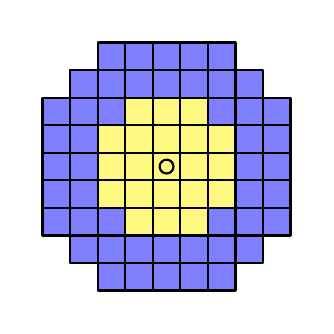
\begin{tikzpicture}[thick,scale=0.35,line join=round,>=latex]
  \foreach \i in {-3,...,3} {
      \foreach \j in {-3,...,3} {
          \printSQ{\i}{\j}{blue!50}
        }
    }
  \foreach \i in {-2,...,2} {
      \printSQ{\i}{4}{blue!50}
      \printSQ{\i}{-4}{blue!50}
      \printSQ{4}{\i}{blue!50}
      \printSQ{-4}{\i}{blue!50}
    }
  
  \foreach \i in {-1,...,1} {
      \foreach \j in {-1,...,1} {
          \printSQ{\i}{\j}{yellow!50}
        }
    }
  \foreach \i in {-1,...,1} {
      \printSQ{\i}{2}{yellow!50}
      \printSQ{\i}{-2}{yellow!50}
      \printSQ{2}{\i}{yellow!50}
      \printSQ{-2}{\i}{yellow!50}
    }
  
  \draw (0,0) circle (0.25);
  \draw [white] (-5,-5) rectangle (5,5);
\end{tikzpicture}
\end{document}